\documentclass[12pt,letterpaper]{article}
\usepackage[utf8]{inputenc}
\usepackage[spanish]{babel}
\usepackage{graphicx}
\usepackage[left=2cm,right=2cm,top=2cm,bottom=2cm]{geometry}
\usepackage{graphicx} % figuras
% \usepackage{subfigure} % subfiguras
\usepackage{float} % para usar [H]
\usepackage{amsmath}
%\usepackage{txfonts}
\usepackage{stackrel} 
\usepackage{multirow}
\usepackage{enumerate} % enumerados
\renewcommand{\labelitemi}{$-$}
\renewcommand{\labelitemii}{$\cdot$}
% \author{}
% \title{Caratula}
\begin{document}

% Fancy Header and Footer
% \usepackage{fancyhdr}
% \pagestyle{fancy}
% \cfoot{}
% \rfoot{\thepage}
%

% \usepackage[hidelinks]{hyperref} % CREA HYPERVINCULOS EN INDICE

% \author{}
\title{Caratula}

\begin{titlepage}
\begin{center}
\large{UNERSIDAD PRIVADA DE TACNA}\\
\vspace*{-0.025in}
\begin{figure}[htb]
\begin{center}

\includegraphics[width=8cm]{./Imagenes/logo}
\end{center}
\end{figure}
\vspace*{0.15in}
INGENIERIA DE SISTEMAS  \\

\vspace*{0.5in}
\begin{large}
TITULO:\\
\end{large}

\vspace*{0.1in}
\begin{Large}
\textbf{INFORME DEL TRABAJO FINAL UNIDAD I} \\
\end{Large}

\vspace*{0.3in}
\begin{Large}
\textbf{CURSO:} \\
\end{Large}

\vspace*{0.1in}
\begin{large}
INTELIGENCIA DE NEGOCIOSI\\
\end{large}

\vspace*{0.3in}
\begin{Large}
\textbf{DOCENTE(ING):} \\
\end{Large}

\vspace*{0.1in}
\begin{large}
 Patrick Cuadros Quiroga\\
\end{large}

\vspace*{0.2in}
\vspace*{0.1in}
\begin{large}
INTEGRANTES: \\
Ordoñez Quilli, Ronald         	 (2015052821)\\
Mamani Ayala, Brandon               (2015052715)\\
Quispe Mamani, Angelo	     	 (2015052826)\\
Vizcarra Llanque, Jhordy	   	 (2015052719)\\
Rodriguez Mamani, Juan     	 (2017057862)\\
\begin{flushleft}
\end{flushleft}
\end{large}
\end{center}

\end{titlepage}


\tableofcontents % INDICE
\thispagestyle{empty} % INDICE SIN NUMERO
\newpage
\setcounter{page}{1} % REINICIAR CONTADOR DE PAGINAS DESPUES DEL INDICE

 \section{Actividad No 01 – Resumen} 
Resumen aqui
 \section{Marco Teorico} 
\subsection{Modelo de Negocios Canvas}
\begin{enumerate}[1.]
	
	\item Modelo de Negocios Canvas
	\\
	\\
	 Para el desarrollo de nuestro modelo de negocios canvas, algunas personas piensan en tener una buena idea, una idea perfecta. Sin embargo, muchos ni siquiera se han tomado el tiempo de validarla con un grupo de personas con necesidades y gustos distintos a los propios. En 2010 Alex Osterwalder diseño el Business Model Canvas: un formato que visualiza el modelo de negocio en una sola hoja con 9 divisiones. Este método resulta en un documento que ofrece una visión global detallada de la idea de negocio, mostrando claramente las interconexiones entre los diferentes elementos.\\
Estas 9 divisiones ayudan a separar todo el flujo de trabajo de la idea que tenemos en mente. Poco a poco vamos a ir estructurándola y dándole sentido. Para tener éxito al desarrollar este modelo para una idea propia, lo primero es conocer y tener un concepto detallado de lo que significa cada sección:\\
		\begin{enumerate}[a)]
			\item Segmento de Cliente \\
			\\
			Se refiere a los grupos de personas a los que se quiere ofrecer el producto o servicio. Son la base del negocio, así que es ideal conocerlos muy bien. Para entenderlos es importante recordar que, en algunos casos, un cliente es quien paga y un usuario es aquel que sólo consume el producto o utiliza el servicio. Un ejemplo práctico sería el de un niño al que su padre le regala un videojuego: el papá es el cliente y el niño es el usuario final.\\

			\item Propuesta de Valor \\
			\\
			Se trata del pain statement que solucionamos para el cliente y cómo le damos respuesta con el producto y/o servicio. La iniciativa debe sobresalir en el mercado, nos debe hacer notar. Este es el valor agregado que nos llevaría al éxito.\\
			\\
			\item Canales de Distribucion \\
			\\
			Se centra en determinar cómo comunicar, alcanzar y entregar la propuesta de valor a los clientes. Estamos en siglo XXI y podemos utilizar el internet para este propósito a través de un sitio web, redes sociales, mailing, centro comercial, etc.\\
			\\
			\item Relaciones con el Cliente \\
			\\
			Es uno de los aspectos más críticos en el éxito del modelo de negocio y uno de los más complejos de hacer tangible. Se pueden establecer diferentes tipos de relaciones, dependiendo del segmento o tipo de cliente. Las relaciones humanas son sumamente importantes. Un ejemplo práctico: redes sociales.\\
			\\
			\item Flujo de Ingreso \\
			\\
			Representa la forma en la que se generan los ingresos por cada cliente. La obtención de ingresos puede ser directa o indirecta, en un sólo pago o recurrente. Debemos analizar muy bien y preguntarnos por qué pagaría el cliente por este producto o servicio y cuál sería su método de pago. En algunos casos se puede utilizar el modelo de pago fremium, que consiste en ofrecer el servicio de manera gratuita (o con uso limitado) por un tiempo. Para, después, ofrecer una mejor experiencia con la condición de pago.\\
			\\
			\item Recursos Clave \\
			\\
			Los recursos más importantes, necesarios para el funcionamiento del negocio. Se clasifican por tipo, cantidad e intensidad. Debemos saber qué vamos a necesitar para llevar a cabo el proyecto. Esto incluye la mano de obra: es importante buscar a las personas adecuadas con el perfil indicado.\\
			\\
			\item Actividades Clave \\
			\\
			Para entregar la propuesta de valor se deben desarrollar una serie de actividades clave internas como:\\
			\\
			- Definir procesos de producción\\
			- Marketing\\
			- Tiempos de desarrollo\\
			- Cronograma de actividades detallado con tiempos y fechas\\
			\\
			\item Red de Asociados\\
			\\
			Se definen las alianzas necesarias para ejecutar el modelo de negocio con garantías. Estas deben complementar las capacidades y optimizar la propuesta de valor: la co-creación es imprescindible hoy en día en los negocios. Una buena idea requiere de una inversión y para ello podemos realizar alianzas con inversionistas o empresas capaces de aportar. En ocasiones, las alianzas no se hacen sólo por obtener un fin económico; sino que el proyecto puede generar beneficios para ambas partes.\\
			\\			
			\item Estructura de Costos\\
			\\
			Describe todos los costos necesarios al operar el modelo de negocio. Se trata de conocer y optimizar el capital para intentar diseñar un modelo de negocio sostenible, eficiente y escalable. Después de seguir este modelo, tendremos una idea de negocio bastante compacta que puede seguir desarrollándose todos los días. Una recomendación es imprimirlo y pegarlo en un lugar visible para que cada que surja una nueva idea, se pueda agregar en la sección que corresponda. Estas ideas pueden validarse en el mercado y desecharse o complementarse. Con el paso del tiempo, tendremos un proyecto completo que puede pasar a la etapa de elaboración o ejecución con plena garantía de que si trabajamos con dedicación, constancia y sacrificio se convertirá en un gran negocio, producto o servicio, innovador y sostenible.\\

		\begin{center}
                    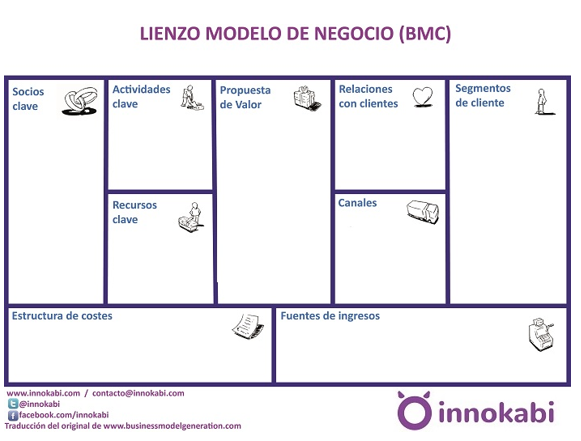
\includegraphics[scale=0.60]{./Imagenes/ang_1}
                    \end{center}

 \subsection{Desarrollo del Modelo Canvas con RENIEC}		
		\end{enumerate}
		
\subsection{Definicion Qlik Sense} 

              \item ¿Qu\'e es Qlink Sense?. \\
               
	   

                     \begin{center}
                    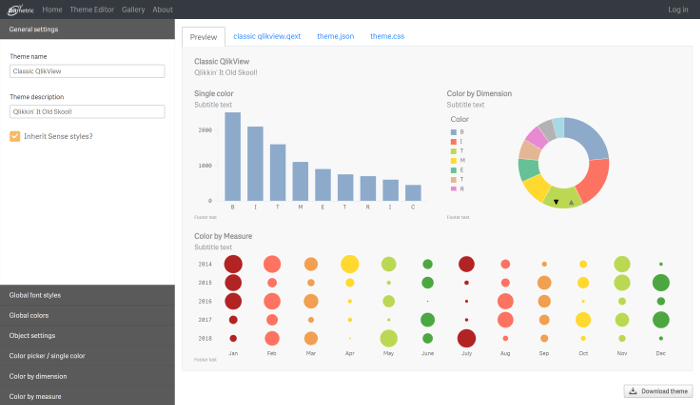
\includegraphics[scale=0.60]{./Imagenes/qlik_sense.png}
                    \end{center}
                
                   Qlik Sense es una aplicaci\'on de visualizaci\'on y descubrimiento de datos gobernada, basada en servidor, ideal para las necesidades anal\'iticas de grupos, departmentos o toda una organizaci\'on. Los usuarios de negocio obtienen un an\'alisis de datos potente, flexible y personalizado y colaboraci\'on en cualquier dispositivo, a la vez que se adhieren a unas pol\'iticas de gobierno y seguridad centralizada de datos.\\
                  \\ 
              \item ¿Como podemos hacer?\\
               \\ 
               La mayor\'ia de productos de Business Intelligence (BI) ayudan a las personas a responder preguntas que ya se comprenden de antemano. Pero ¿qu\'e ocurre con las preguntas que se nos van ocurriendo despu\'es o sobre la marcha? ¿Ese tipo de preguntas que surgen tras leer un informe o visualizar un grafico? Con la experiencia asociativa de Qlik Sense, podemos hacer todas las preguntas que se nos ocurran y responderlas una tras otra, avanzando por nuestra propia ruta hacia el conocimiento. Con Qlik Sense podemos explorar los datos libremente, mediante simples clics de rat\'on, aprendiendo y profundizando en cada etapa del camino y descubriendo nuevas rutas de exploraci\'on basadas en nuestros propios descubrimientos.
              \\
              \\
               \\
               \\
              \item Utilidades \\
            \\
A trav\'es de visualizaciones inteligentes puedes: \\
             
                \begin{center}
                    
\includegraphics[scale=0.60]{./Imagenes/caracteristicas.png}
                 \end{center}

        \begin{itemize}
         \item Transmitir el significado de los datos con visualizaciones inteligentes, innovadoras, completamente interactivas y con capacidad de reacci\'on.\\
         \item Explorar en cualqxuier direcci\'on: encuentrar datos e informaci\'on valiosa que las herramientas jerarquicas y basadas en consultas no detectan.\\
         \item Lograr una flexibilidad absoluta: solo tienes que escribir lo que necesites para encontrar información relacionada y ver datos relacionados en todo el conjunto de datos.\\
          \item Explorar m\'ultiples fuentes de datos: conectar y visualizar datos de varias fuentes para una vista m\'as exhaustiva.\\
          \item Narraci\'on de datos detallada: colaborar y compartir la informaci\'on extraida del an\'alisis visual. Comunicar mejor los hallazgos a su equipo. Moverte directamente entre historias y an\'alisis en directo para responder a preguntas y acelerar la toma de decisiones.\\
        \end{itemize}

         \item  Caracteristicas 
    
       \begin{description}
            \item[Multifuente:] Se conecta con m\'ultiples fuentes de datos, incluyendo entradas de datos en tiempo real, a fin de proporcionar unas vistas aun m\'as exhaustivas, sin comprometer el rendimiento de las aplicaciones.\\
            \item[Colaborativo:] La funcionalidad de Qlik Sense le permitir\'a una narraci\'on de datos facil con la que podra compartir el análisis de una forma visual, comunicar sus hallazgos a los equipos y colaborar con mayor eficacia.\\
            \item[AutoServicio:] Cualquier usuario puede crear sus propias visualizaciones de datos, sus cuadros de mando, al tiempo que ofrece a TI la confianza de estar diseñando unas librerías seguras y consistentes y unos datos bien gobernados.\\
            \item[DragandDrop:] Las visualizaciones inteligentes, en combinaci\'on con los datos Qlik patentados de su motor de indexaci\'on, descubren todas las relaciones entre las dimensiones de datos, revelando conocimientos que habr\'ian permanecido ocultos en los modelos tradicionales de datos basados en consultas y jerarqu\'ias. Datos, informacion y conocimiento.\\

        \end{description}
               


    
\end{enumerate}

 \section{Desarrollo} 

Para realizar la demostracion de la funcionalidad de está herramienta,  es necesario realiza los siguientes pasos previos para su aplicación.
\subsection{Instalar herramienta Qlik Sense}

Es necesario para poder realizar esta prueba es necesario saber como instalar esta herramienta , es muy facil e intuitiva los pasos son: 

\begin{itemize}
		\item Ejecutar el instalador como modo administrador, una vez desplegada la ventana. Seleccionaremos la opcion instalar.
\begin{center}
	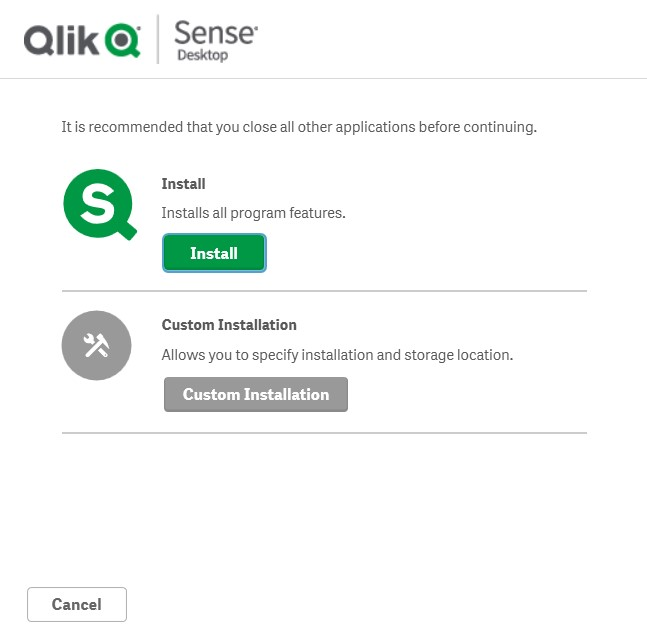
\includegraphics[width=10cm]{./Imagenes/img1} 
\end{center}
		\item Aceptaremos las licencias de la herramienta y daremos siguienta.
\begin{center}
	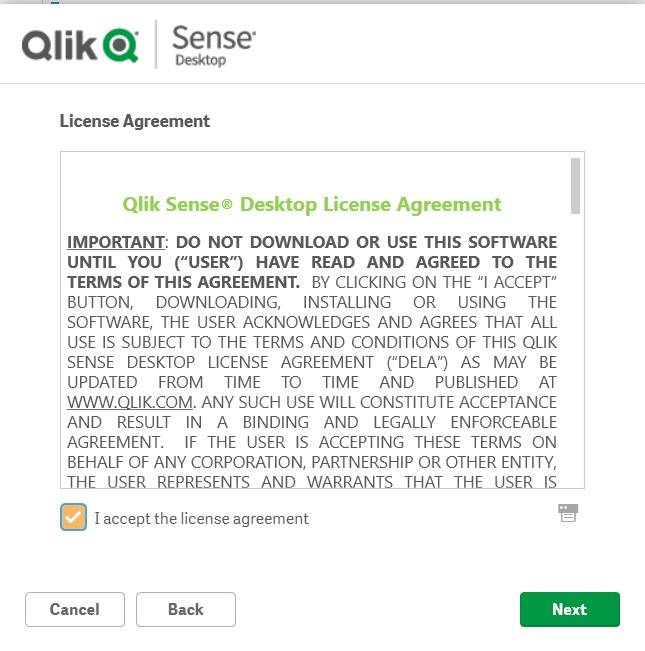
\includegraphics[width=10cm]{./Imagenes/img2} 
\end{center}
		\item Pulsamos el botón «Instalar».
\begin{center}
	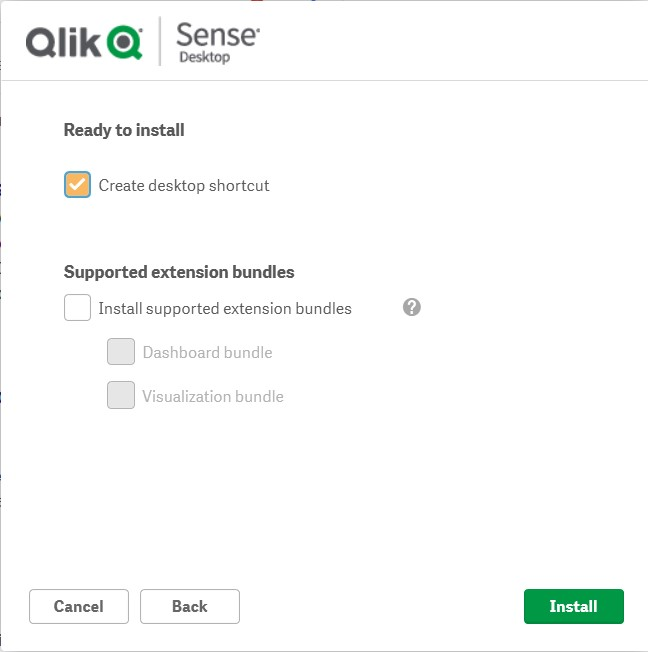
\includegraphics[width=10cm]{./Imagenes/img3} 
\end{center}
\item Esperamos que se complete la instalacion.
\begin{center}
	
\includegraphics[width=10cm]{./Imagenes/img4} 
\end{center}
\item Y tenemos la aplicacion lista para logearnos.
\begin{center}
	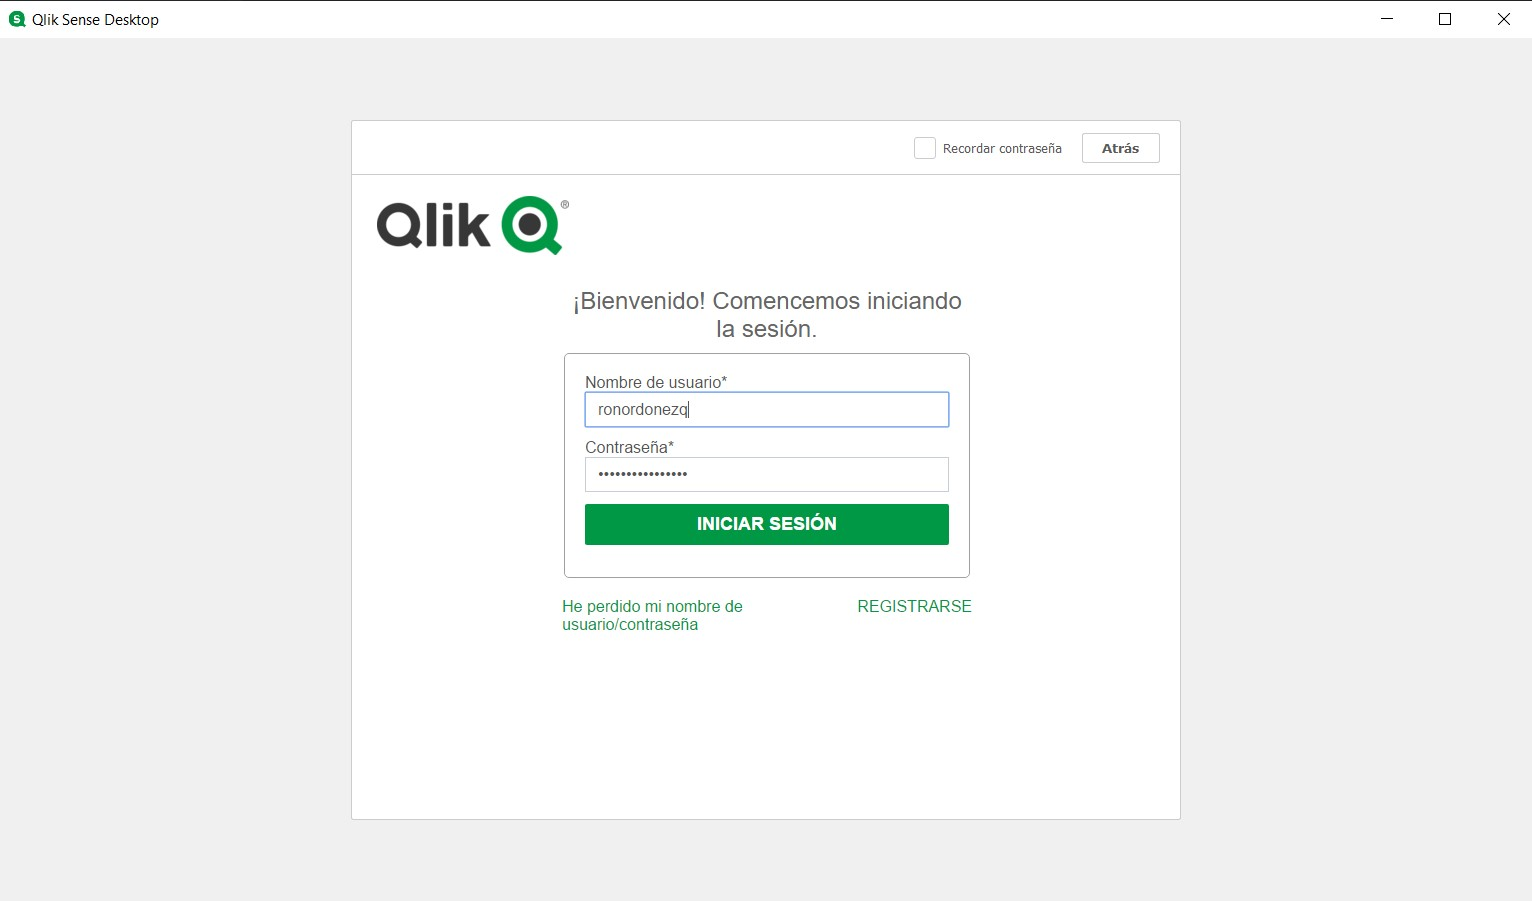
\includegraphics[width=10cm]{./Imagenes/img6} 
\end{center}
\end{itemize}

\subsection{Cargar datos con Qlik Sense}

Lo primero que necesitamos saber para empezar a trabajar con Qlik Sense es saber como cargar nuestra fuente de datos, en este caso vamos a hacerlo paso a paso de una forma bastante detallada. La instalación es verdaderamente sencilla así que pasaremos por alto este paso, solo hay que dar siguiente a todas las ventanas y esperar que la barra de progreso se llene, como es usual en la mayoría de aplicaciones en Windows.
Una vez que tengamos instalado e iniciamos Qlik Sense, lo primero que nos aparecerá es la pantalla de bienvenida:


\begin{center}
	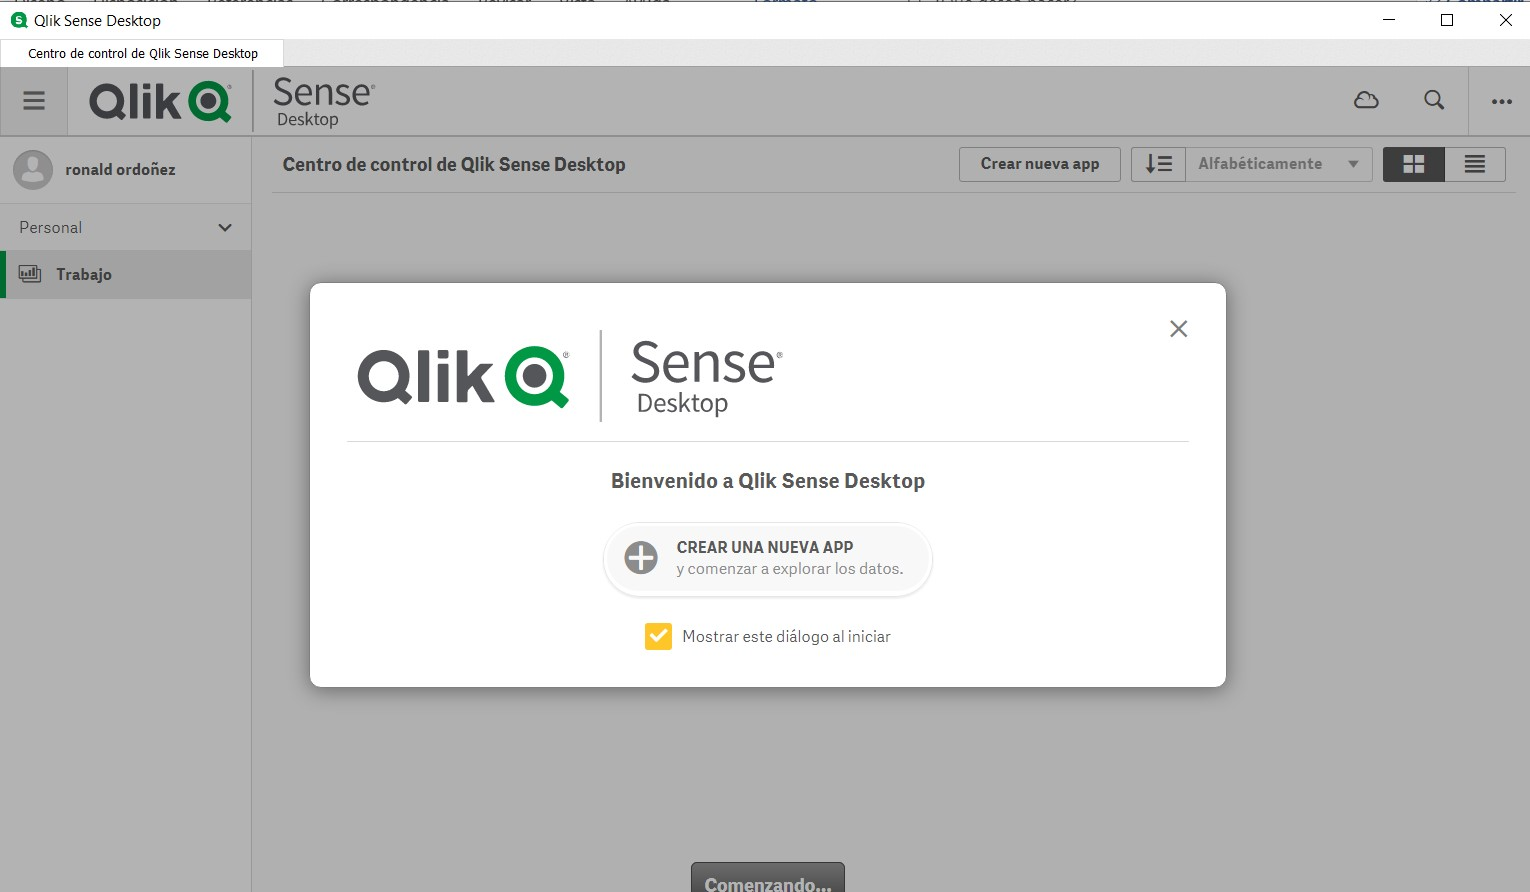
\includegraphics[width=12cm]{./Imagenes/img8} 
\end{center}

Desde aquí deberemos elegir la opción «Crear una nueva App», a continuación se nos pedirá ingresar el nombre para la nueva aplicación que vamos a crear, en mi caso le puse como nombre «TestLoad» y luego pulsar en el botón «Crear».

\begin{center}
	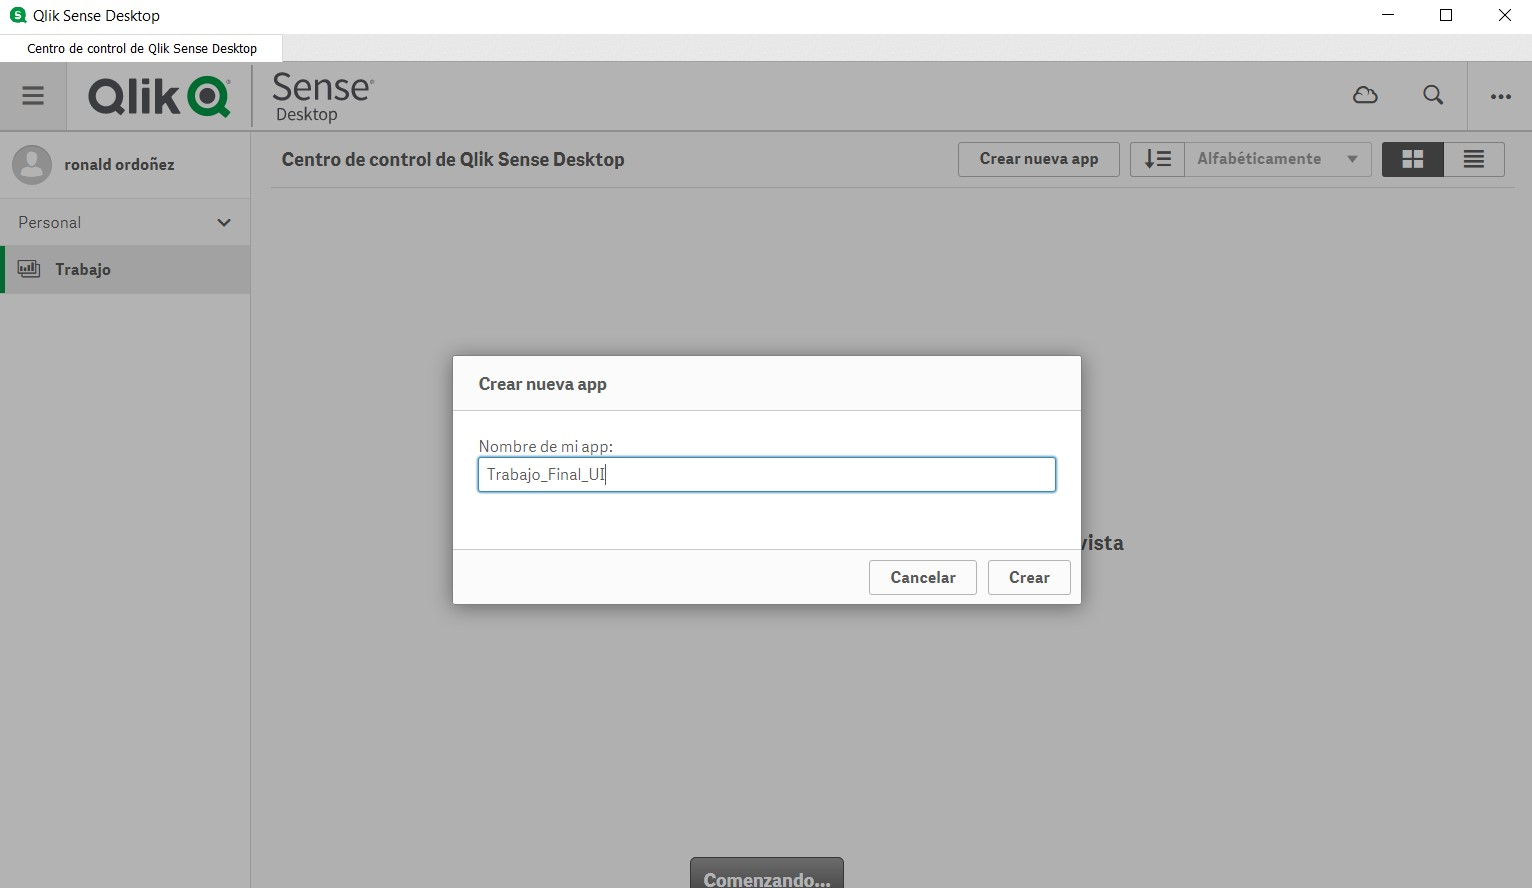
\includegraphics[width=12cm]{./Imagenes/img9} 
\end{center}

En la siguiente vista sólo nos mostrará un mensaje indicando que nuestra app fue creada satisfactoriamente. Ahora pulsar en el botón «Cancelar».
\begin{center}
	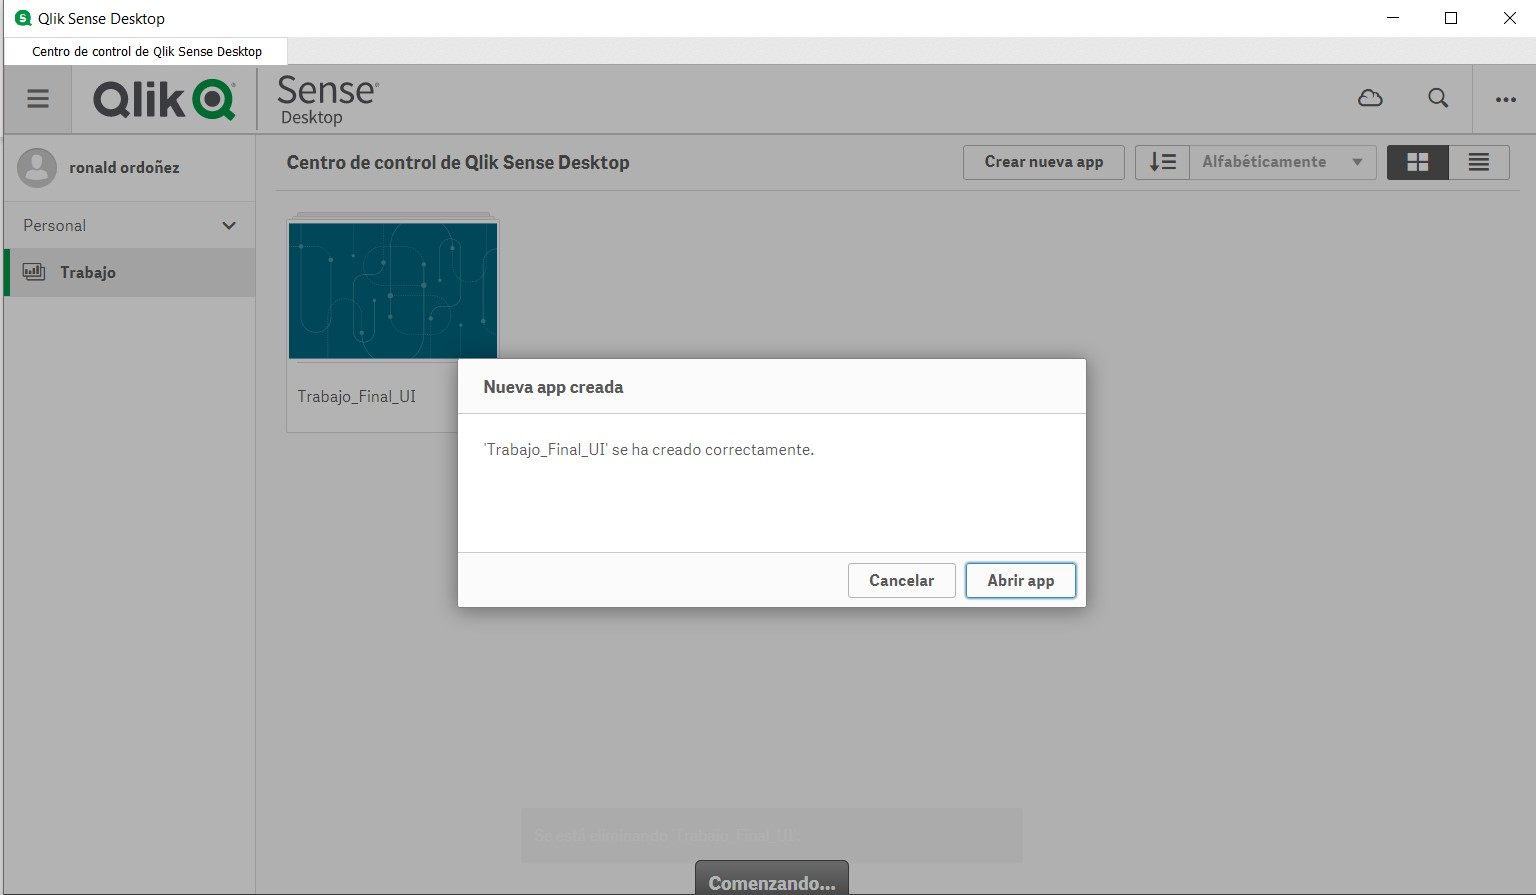
\includegraphics[width=12cm]{./Imagenes/img10} 
\end{center}

A continuación podremos visualizar las dos opciones que nos brinda el Qlik Sense Desktop para poder cargar datos a nuestra aplicación. Estas opciones son:

\begin{itemize}
		\item Añadir datos de archivos y otras fuentes, ya sean estos archivos delimitados por comas (csv, txt, tab, qvo, mem, skv, prn, log), archivos excel (xls, xlw, xlsx, xlsm), archivos HTML (html, htm, php), archivos KML, archivos de registro fijo (fix, dat), archivos de datos QlikView (qvd), archivos de intercambio de datos QlikView (qvx) o archivos XML.
		\item Editor de script, desde esta opción se tendrá acceso al script de nuestra aplicación, desde donde podremos conectarnos a archivos o bases de datos y realizar el proceso de transformación de datos.
Para esta demostraciòn elegir la primera opción «Añadir datos de archivos y otras fuentes».
\end{itemize}


\begin{center}
	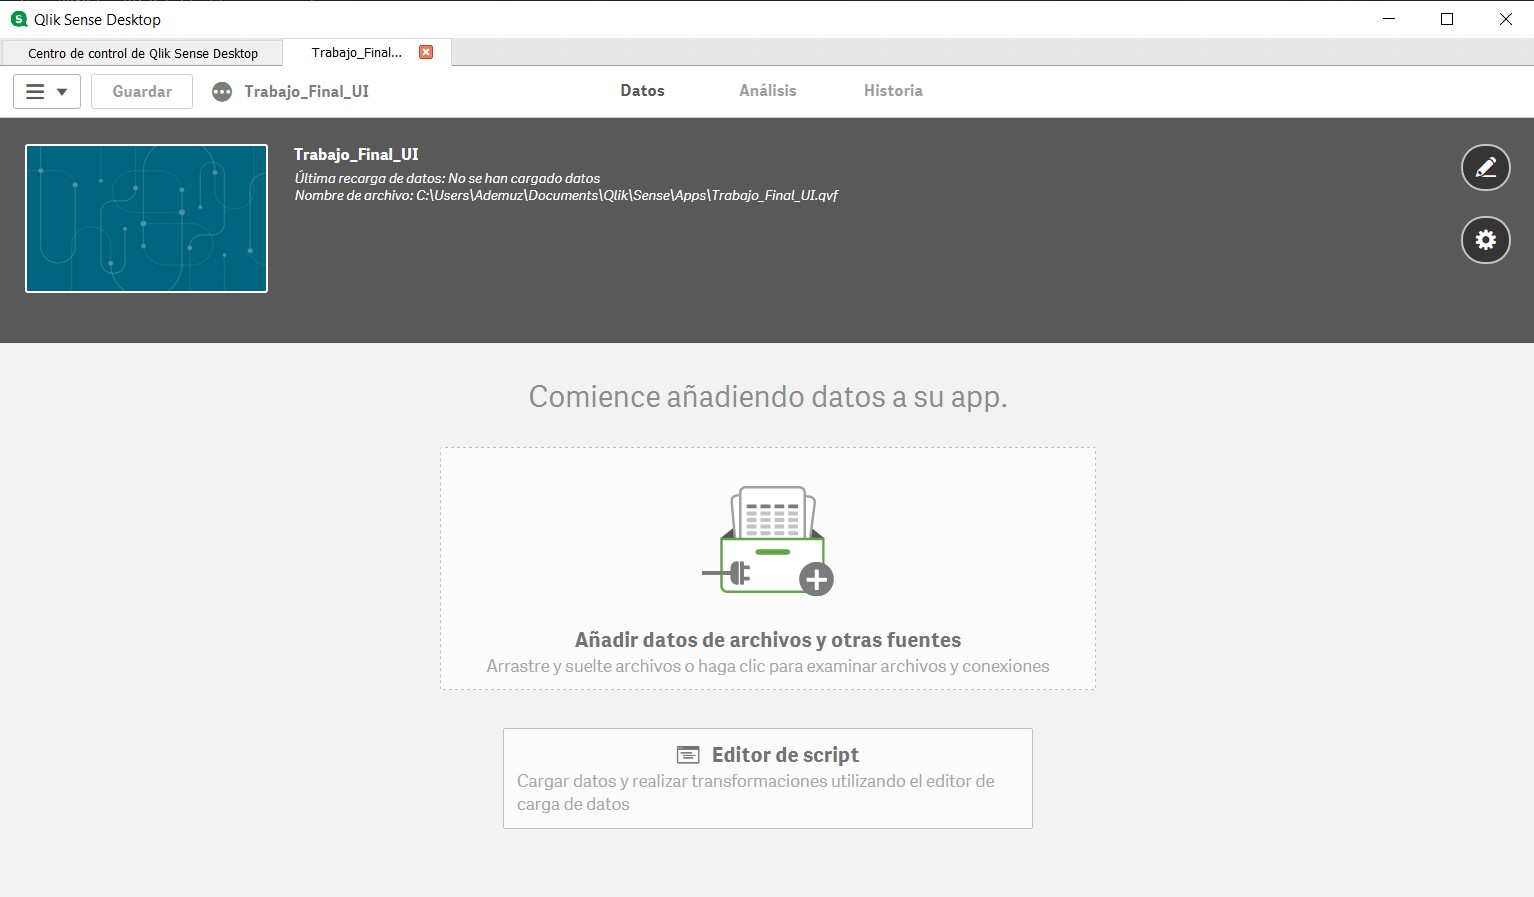
\includegraphics[width=12cm]{./Imagenes/img11} 
\end{center}


Ahora el asistente pedirá ubicar el archivo que se desea cargar, en mi caso voy a tomar un Qvd el cual ya fue procesado en un proyecto anterior. \\
En la siguiente vista, se podrá visualizar una muestra de los datos a cargar y los nombres de sus campos.
Por defecto aparece marcado el check que dice «Seleccionar todos los campos», con lo cual se cargará todas las columnas a nuestra aplicación. En caso no se desee cargar todo, se puede marcar/desmarcar el check que tiene cada columna y de esta forma dejar solo las que se necesita.

\begin{center}
	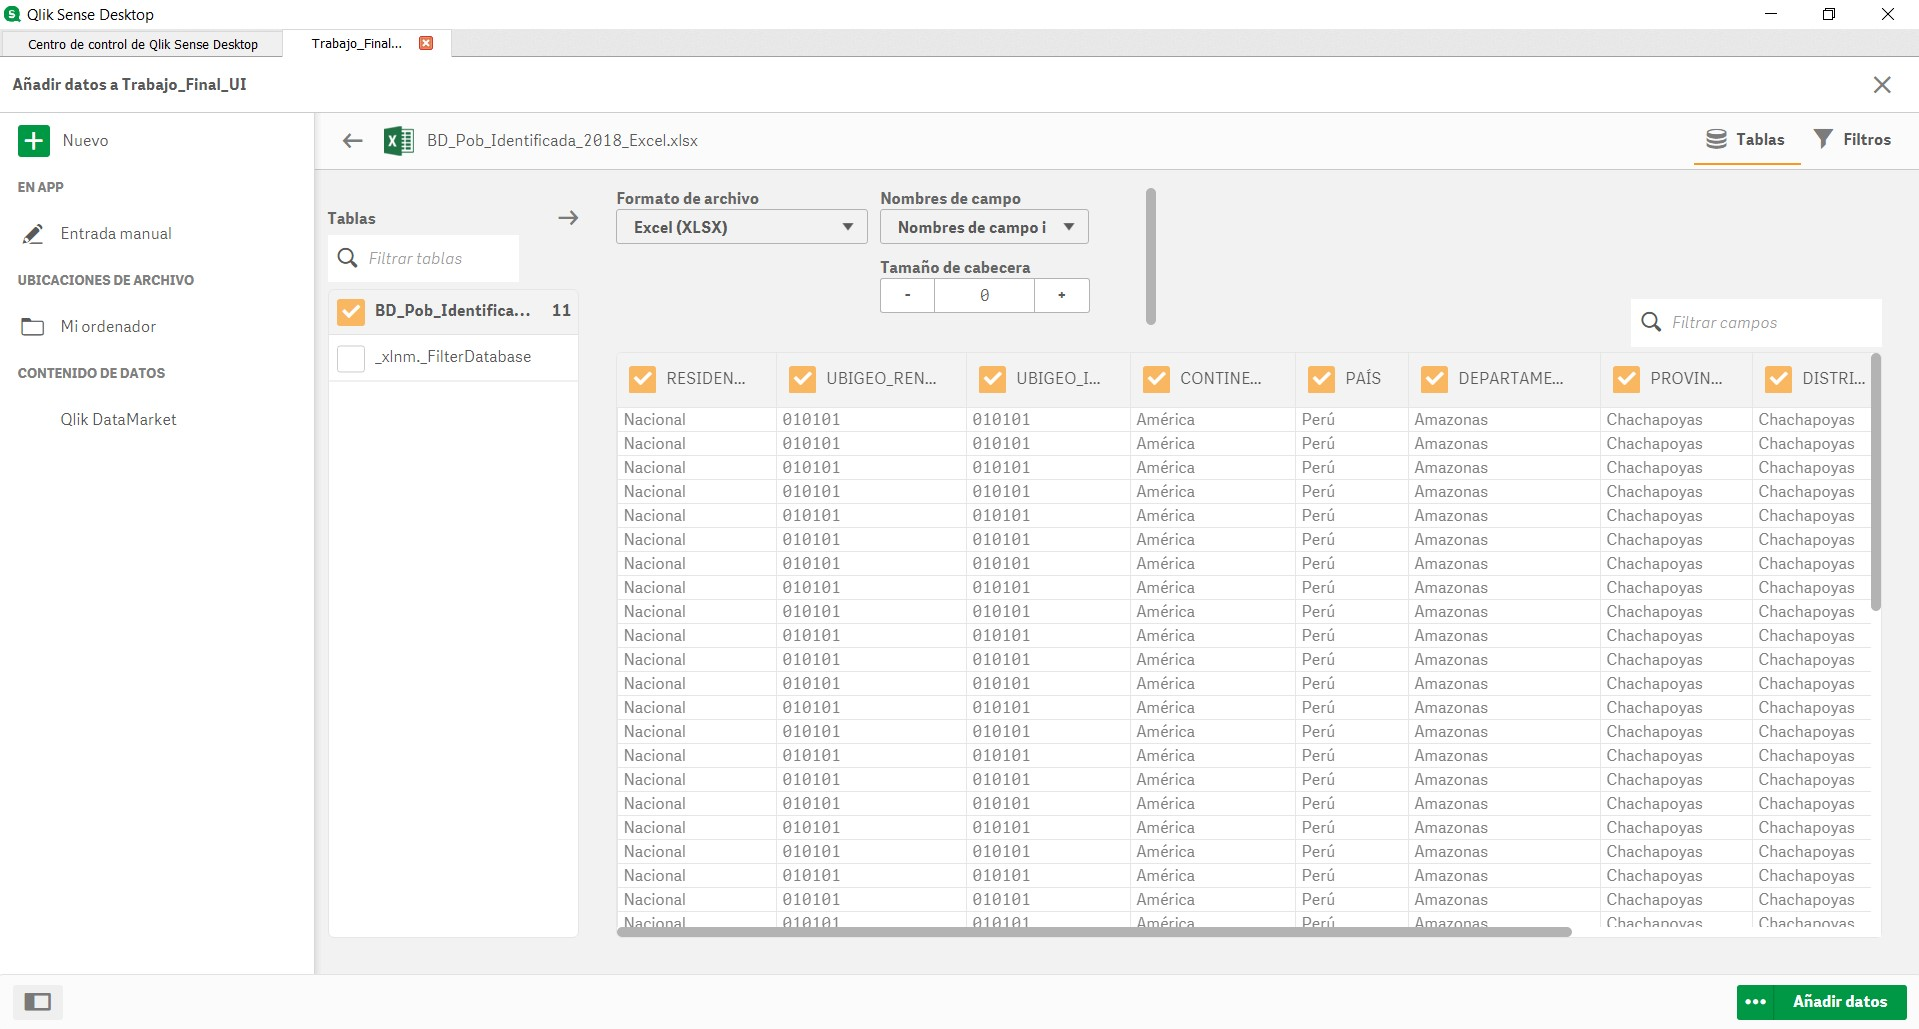
\includegraphics[width=12cm]{./Imagenes/img12} 
\end{center}

La carga como es usual cuando trabajamos con archivos excel será bastante rápida y una vez terminada nos aparecerá la siguiente ventana indicando el tiempo que ha tomado realizar la carga, en esta ventana solo pulsar «Cerrar» para poder.

\begin{center}
	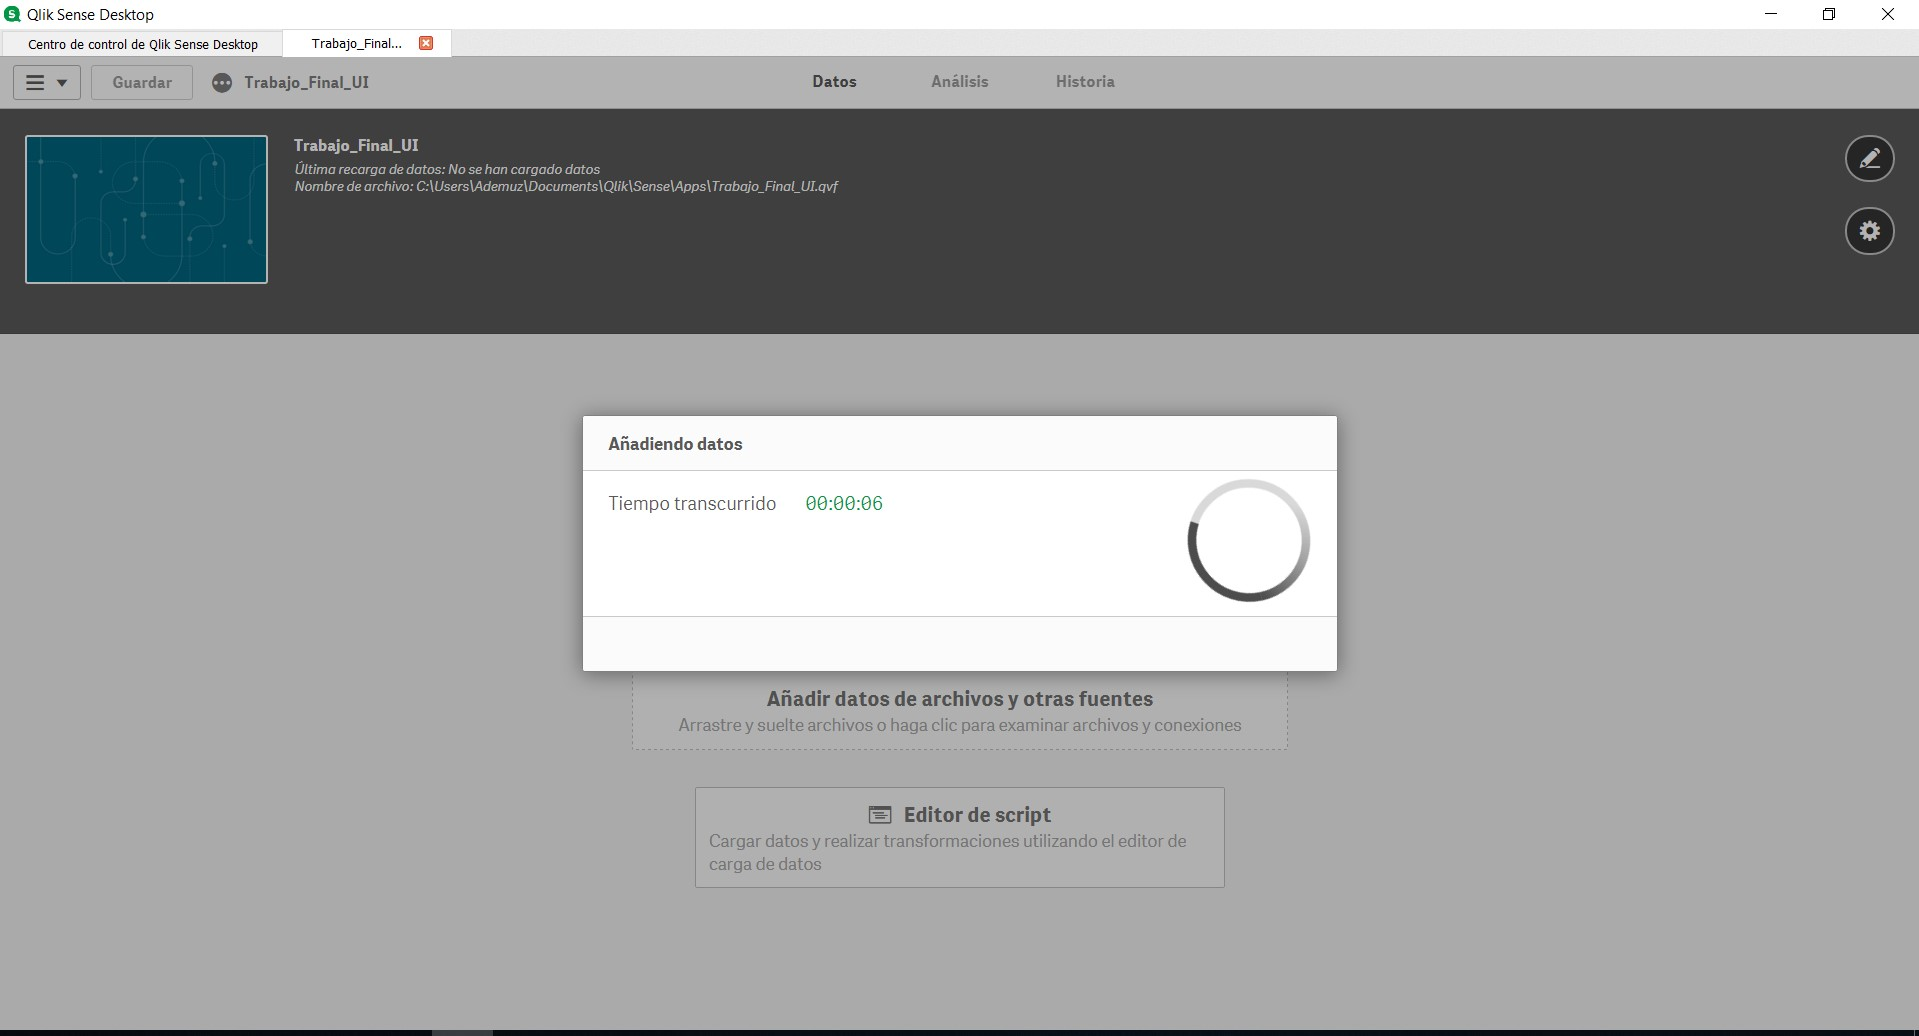
\includegraphics[width=12cm]{./Imagenes/img13} 
\end{center}

Luego de esto estaremos en nuestra aplicación como tal, vamos a revisar las opciones que tenemos disponibles en los menús, en el primero se ve como deshabilitado el botón de «Vista general de app», ya que es justo donde nos encontramos.
\begin{center}
	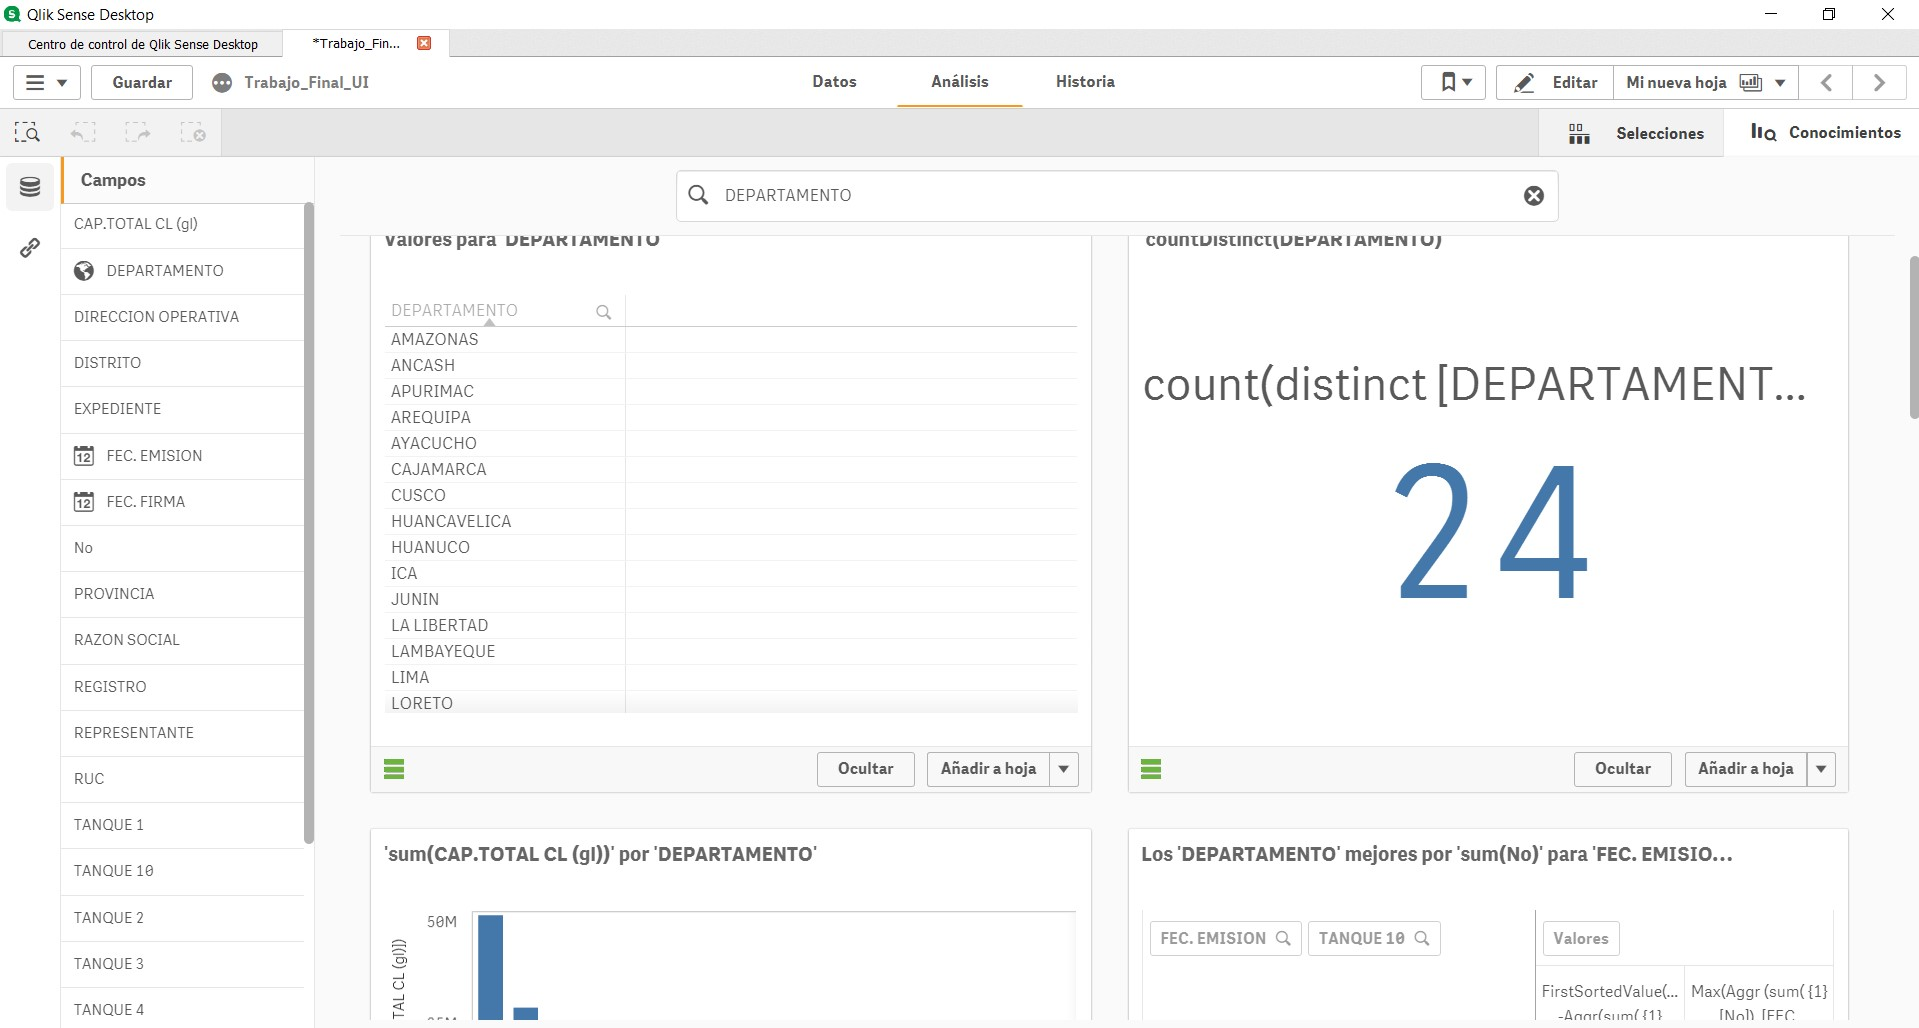
\includegraphics[width=12cm]{./Imagenes/img14} 
\end{center}

\subsection{Resultados generados}


\begin{center}
	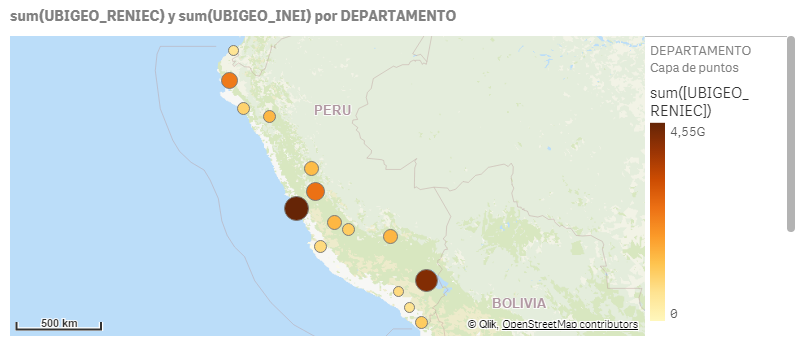
\includegraphics[width=12cm]{./Imagenes/imgDesarrollo_1} 
\end{center}

\begin{center}
	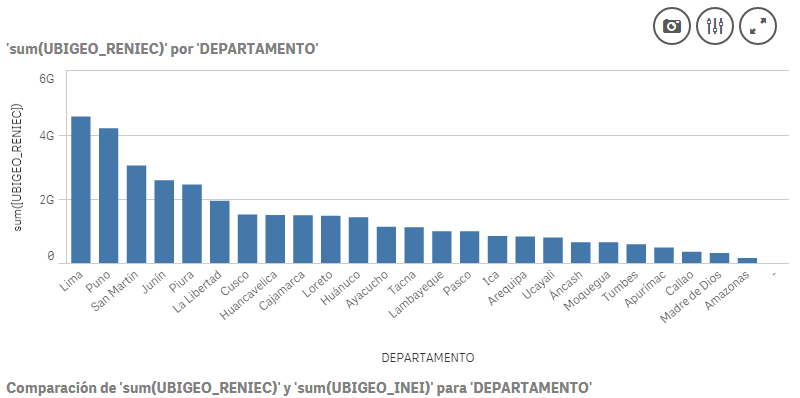
\includegraphics[width=12cm]{./Imagenes/imgDesarrollo_2} 
\end{center}

\begin{center}
	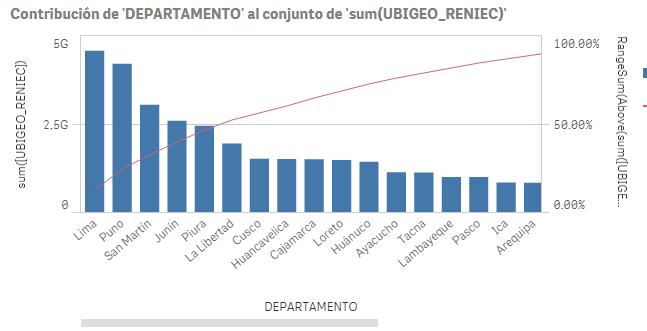
\includegraphics[width=12cm]{./Imagenes/imgDesarrollo_3} 
\end{center}

\begin{center}
	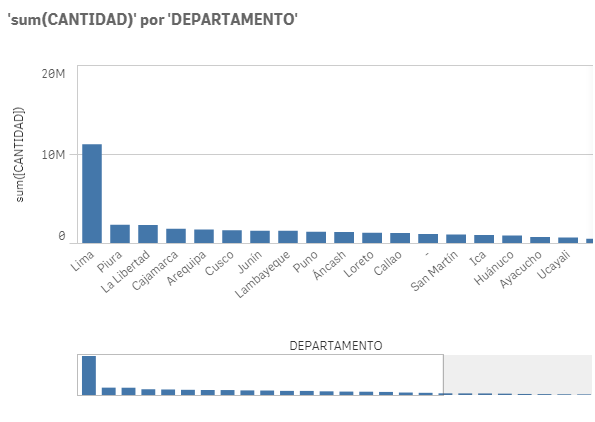
\includegraphics[width=12cm]{./Imagenes/imgDesarrollo_4} 
\end{center}

\begin{center}
	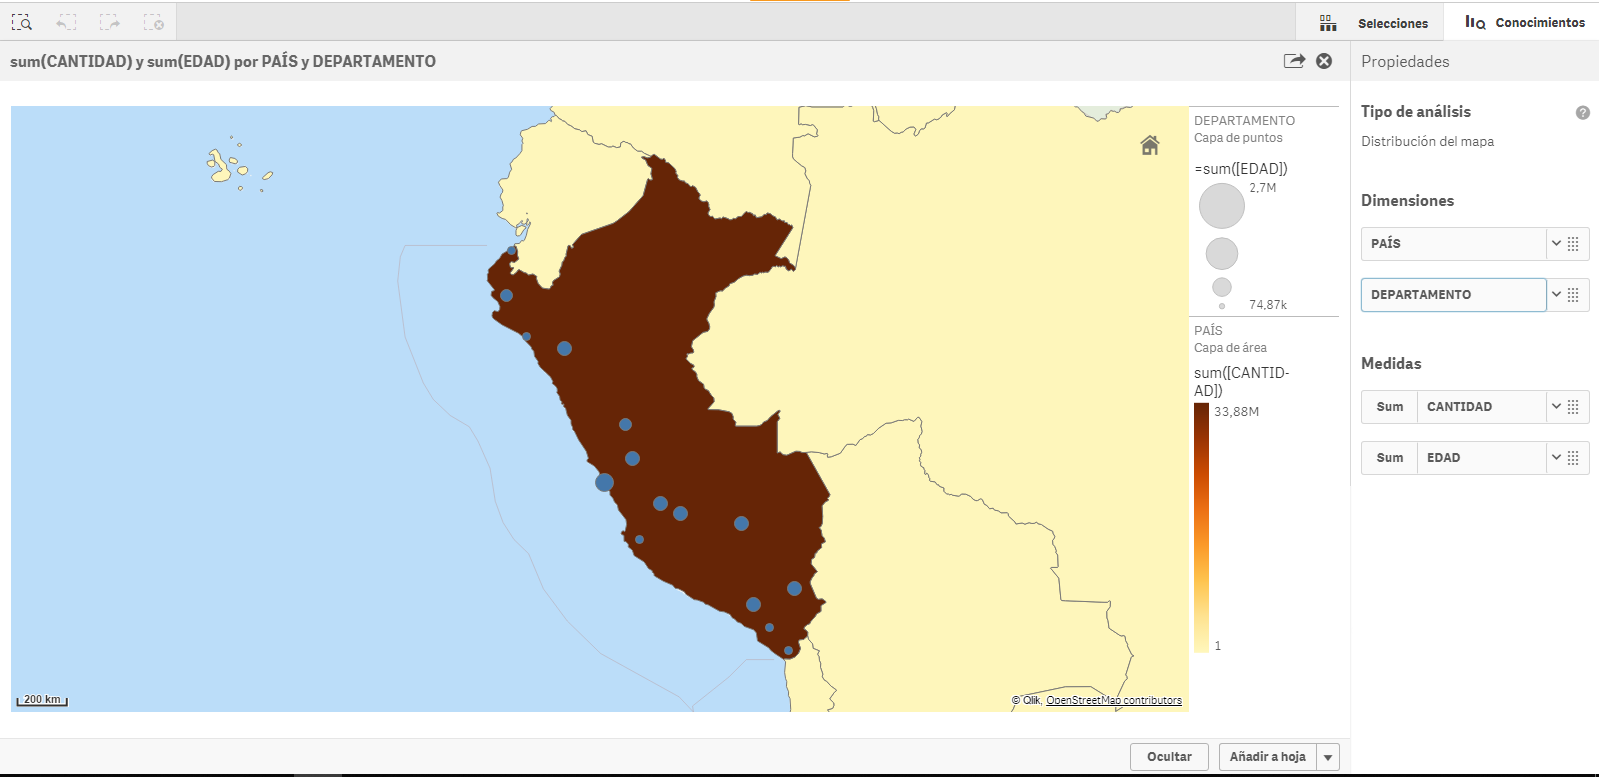
\includegraphics[width=12cm]{./Imagenes/imgDesarrollo_5} 
\end{center}

\begin{center}
	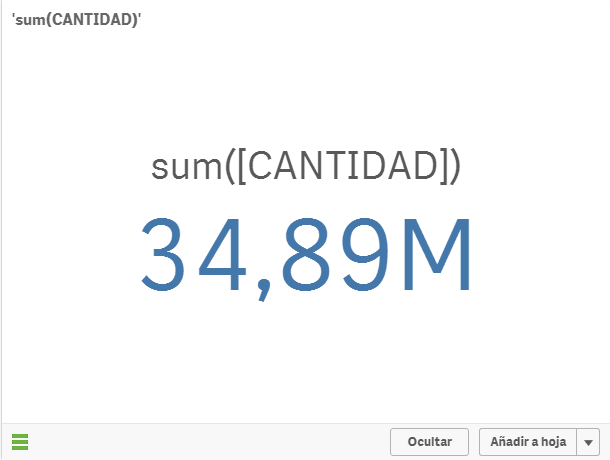
\includegraphics[width=12cm]{./Imagenes/imgDesarrollo_6} 
\end{center}

\begin{center}
	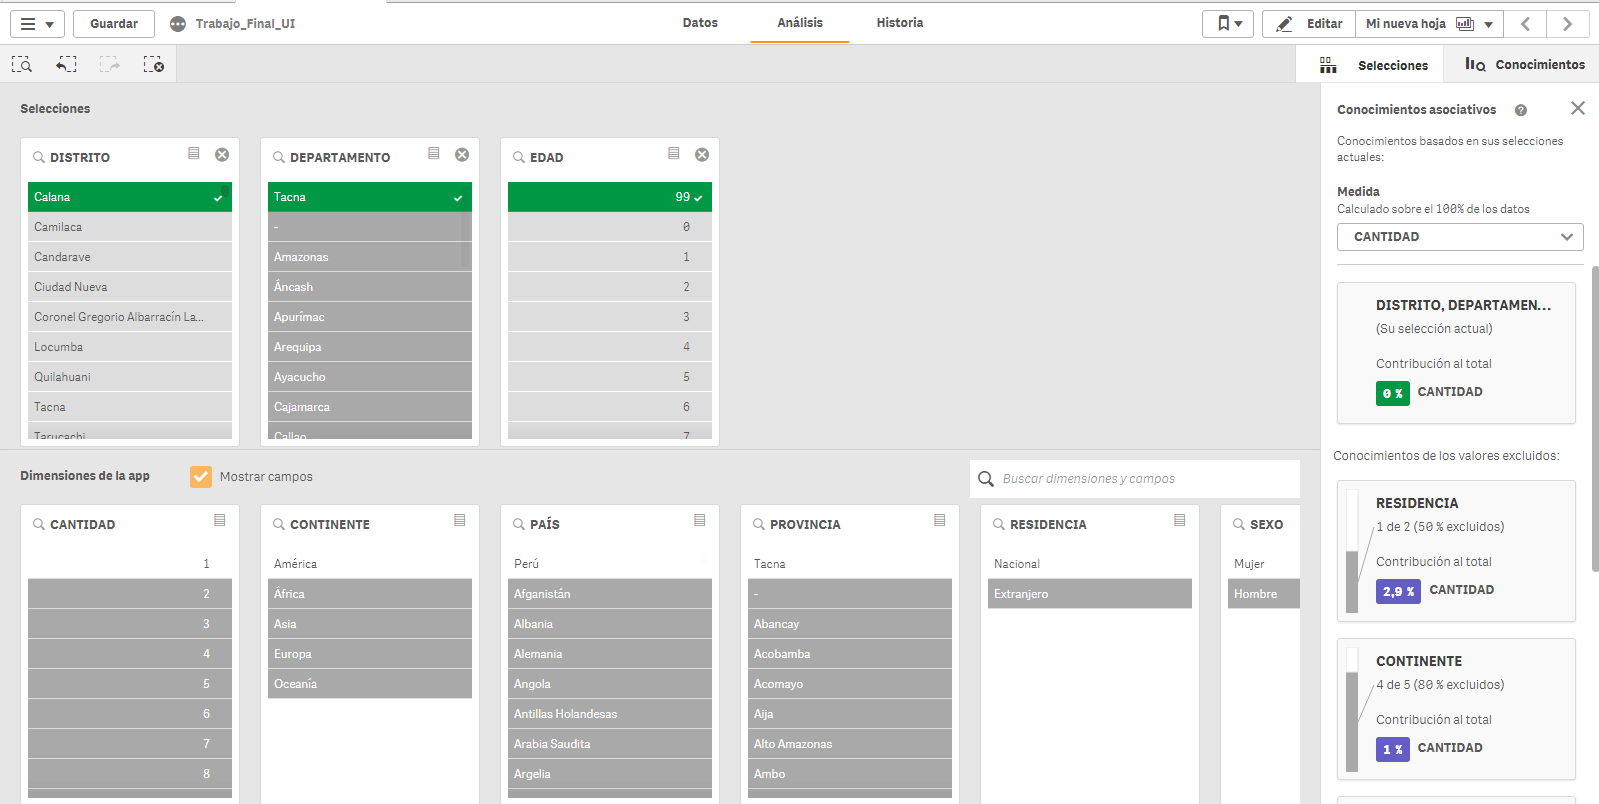
\includegraphics[width=12cm]{./Imagenes/imgDesarrollo_7} 
\end{center}
 \section{Bibliografía} 
Aqui bibliografía



\end{document}
